\chapter{Decoding问题}

\textsl{Decoding问题}就是在给定观测序列的情况下,寻找最大概率可能出现的隐概率状态序列,即
\begin{equation}
    \hat{I}=\arg\max_{I}P(I|O,\lambda)
\end{equation}

\section{Decoding}

首先画出HMM拓扑模型

\begin{figure}[H]
    \centering
    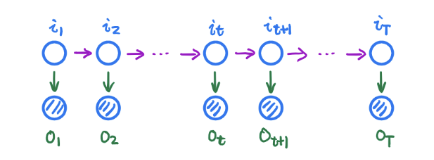
\includegraphics[scale=0.6]{figures/Hidden-Markov-model-Topology.png}
    \caption{Hidden Markov Model拓扑模型}
\end{figure}

我们要看$o_t$的的概率分别是多少时$i_t$的概率最大,这里实际上就是一个动态规划问题,只不过将平时的最大距离问题等价于最大概率问题,
每个时刻都有$N$个状态,从$N^T$个可能的序列中找出概率最大的排列

\begin{figure}[H]
    \centering
    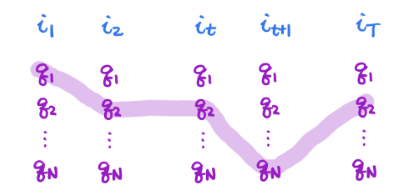
\includegraphics[scale=0.6]{figures/动态规划问题.png}
    \caption{Hidden Markov Model Decoding的动态规划}
\end{figure}


\section{Viterbi Algorithm}

我们假设
\begin{equation}
    \delta_t(i)=\max\limits_{i_1,\cdots,i_{t-1}}\ P(o_1,\cdots,o_t,i_1,\cdots,i_{t-1},i_t=q_i)
\end{equation}

这个等式的意思是,假设前面$t-1$个时刻随便走,第$t$个时刻走到$q_i$,从中选取概率最大的序列,我们下一步的目标就是在知道$\delta_t(i)$的情况下如何求$\delta_{t+1}(i)$

\begin{figure}[H]
    \centering
    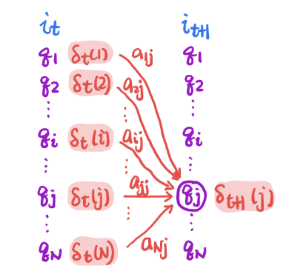
\includegraphics[scale=0.6]{figures/V.png}
    \caption{Viterbi算法示意图}
\end{figure}

\begin{equation}
    \begin{aligned}
        \delta_{t+1}(j)&=\max\limits_{i_1,\cdots,i_T}\ P(o_1,\cdots,o_{t+1},i_1,\cdots,i_t,i_{t+1}=q_j)\\
        &=\max\limits_{i_1,\cdots,i_T}\ \delta_t(i)\cdot a_{ij}\cdot b_j(o_{t+1})
    \end{aligned}
\end{equation}

这就是Viterbi算法,但是这个算法最后求的是一个值,但没有办法求路径,如果想要求路径,需要引入一个变量
\begin{equation}
    \varphi_{t+1}(j)=\arg\max_{1\leqslant t\leqslant N}\delta_t(i)\cdot a_{ij}\cdot b_j(o_{t+1})
\end{equation}

这个函数用来记录每一次迭代过程中经过的状态index,最终得到
\begin{equation}
    \{\varphi_1,\varphi_2,\cdots,\varphi_T\}
\end{equation}